\documentclass[11pt]{beamer}
\usetheme{Copenhagen}
\usepackage[utf8]{inputenc}
\usepackage{amsmath}
\usepackage{amsfonts}
\usepackage{amssymb}
\usepackage{graphicx}
\usepackage[backend=bibtex,style=ieee]{biblatex}
\addbibresource{abe-blockchain.bib}
\author{Andrei Cristian}
\title{Using ABE to Secure Blockchain Transaction Data}
\setbeamercovered{transparent} 
\setbeamertemplate{navigation symbols}{} 
%\logo{} 
%\institute{} 
%\date{} 
%\subject{} 
\begin{document}

\begin{frame}
\titlepage
\end{frame}

\begin{frame}{Table of Contents}
\tableofcontents
\end{frame}

\section{Introduction}
\begin{frame}{Introduction}
\begin{itemize}
	\item Blockchain technology is increasingly being adopted as a trusted platform to support business functions including trusted and verifiable transactions, tracking, and validation.
	\item Most business use-cases require privacy and confidentiality for data and transactions $\Rightarrow$ \textbf{Private blockchain solutions} $\Rightarrow$ Unable to take full advantage of the capabilities, benefits and infrastructure of public blockchain systems.
	\item \textbf{Attribute-Based Encryption} security solution built on private-over-public (PoP) blockchain $\Rightarrow$ Businesses will be able to \textbf{restrict access}, \textbf{maintain privacy}, \textbf{improve performance}, while still being able to benefit from the distributed trust of public blockchains.
\end{itemize}
\end{frame}

\begin{frame}[allowframebreaks]{Public and Private Blockchains}
\begin{itemize}
	\item Similarities\cite{jayachandran}:
	\begin{enumerate}
		\item both are decentralized peer-to-peer networks, where each participant maintains a replica of a shared append-only ledger of digitally signed transactions;
		\item both maintain the replicas in sync through a protocol referred to as consesnsus;
		\item both provide certain guarantees on the immutability of the ledger, even when some participants are faulty or malicious.	
	\end{enumerate}
	\item The main distinction between public and private blockchain is related to who is allowed to participate in the network.
	\item One of the drawbacks of the public blockchain is the substantial amount of computational power to maintain a distributed ledger at a large scale to achieve consensus, in which each node in a network must solve a complex, resource-intensive cryptographic problem - called Proof of Work (PoW)\cite{nakamoto2008} to ensure all are in sync.
	\item Another disadvantage is the openness of public blockchain, which implies little to no privacy protection for transactions and only supports a weak notion of security.
	\item Many people believe private blockchains could provide solutions to many financial enterprise problems, that public blockchains do not, such as abiding by regulations such as Health Insurance Portability and Accountability Act (HIPPA), anti-money laundering (AML) and know-your-customer (KYC) laws, etc.
	\item Private blockchain is usually much faster, cheaper and respects the company's privacy.
	\item  Private blockchains also provide more control power over the participants in the blockchain.
	\item \textbf{Cross-chain} functionality aims to combine the best features of different blockchain systems\cite{liebkind2018}, both private and public, for the purposes of exchanging value across disconnected ecosystems.
	\item None of existing solutions clearly addressed the problem of applying access control policies to enforce data privacy protection on transaction secrets.
	\item For example, when using smart contract solutions, e.g. Ethereum\cite{ethereumweb}, for procurement in supply-chain, transaction parameters such as product name, quantity, price, purchasing terms, shipping options, address, etc. could all be \textbf{sensitive business secrets}. They should be only viewable for relevant stakeholders. 				\item Hyperledger\cite{cachin2016} addresses this problem by relying on a TA approach to build permission groups for data access control. However, data access must be \textbf{predefined} which is not suitable for complex and dynamic businesses logic that require dynamic access control.
	\item \textbf{RBAC} is \textbf{incompatbile} with the distributed nature of blockchain operations where transaction data are mobile and shared by multiple blockchain participants.
\end{itemize}

\end{frame}

\begin{frame}{POP architecture}

\begin{figure}[!ht]
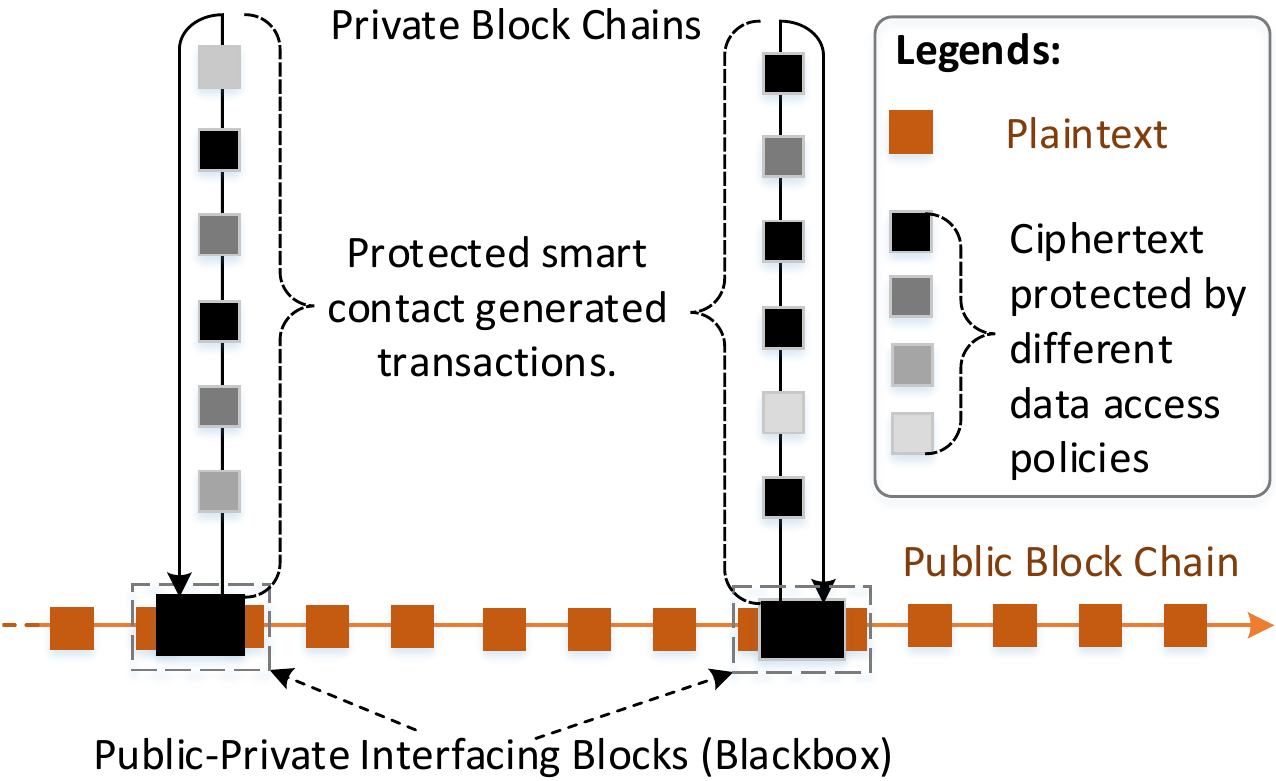
\includegraphics[scale=0.25]{pop.png}
\caption{Illustration of PoP blockchain architecture.}
\label{fig:poparchitecture}
\end{figure}

\end{frame}

\begin{frame}[allowframebreaks]{ABE over PoP Blockchain}
\begin{itemize}
	\item PoP architecture is presented in Figure \ref{fig:poparchitecture}.
	\item Applying ABE on an off-chain basis means it can inter-operate with the public blockchain without interference.
	\item  Private blockchains transactions can be much
\textbf{less computationally intensive} and provide \textbf{superior performance} since they do not have to be verified by all participants.
	\item Businesses are able to choose the private blockchain solution that \textbf{best suits their needs} independently from the public blockchain.
	\item Each private blockchain can be viewed as a \textbf{protected state channel}.
	\item The integrity of a private blockchain can be validated and checked in ciphertext and in aggregate by all public blockchain participants.
	\item The public blockchain infrastructure is leveraged to provide \textbf{validation} and \textbf{immutability} for the entirety of the private blockchain state channel.
	\item This can take
the form of the final private blockchain transaction result, or a hash of the entire private blockchain $\Rightarrow$ distributed trust on the public chain is \textbf{not necessary} for the private blockchain.
	\item \textbf{ABE} provides \textbf{data privacy} for the private blockchain state channel.
	\item Only participants with the appropriate permissions and corresponding ABE attribute private keys can view and validate their relevant blocks in the private block chain.
	\item It provides the benefits of private blockchains in terms of privacy without requiring the deployment of trusted nodes or multiple verification nodes.
	\item It essentially minimizes the entry cost businesses in adopting blockchain solutions.
\end{itemize}
\end{frame}

\begin{frame}[allowframebreaks]{The PoP Solution}
In summary, the presented PoP solution has the following main features:
\begin{itemize}
	\item It is a decentralized trust model for key management of ABE-based data access control. Using this approach, it can incorporate access control policies into ciphertext to protect content of smart contracts.
	\item It is a privacy-preserving messaging protocol to allow private blockchain participants to interact with the smart contract that can generate a private blockchain. This chapter illustrates how to use this protocol based on a supply-chain procurement application.
	\item The solution provides two smart contracts: \textbf{PPP} (Public Parameters and Policies) to establish attribute based security trust model and \textbf{ppSCM} to provide secure data access control based on ABE scheme.
	\item A comprehensive security and performance analysis is presented based on the presented PPP scheme. The presented solution is practical that can significantly reduce the effort and cost to establish dedicated and isolated private blockchains.


\end{itemize}

\end{frame}

\section{System and Models}
\begin{frame}{System and Models}
\begin{itemize}
	\item To illustrate the presented solution, in Figure \ref{fig:supplychain} it is used a supply chain example based on \textbf{Block-Chain Technology}(BCT), which involves multiple parties.
	\item The potential of having all the information written in a blockchain allows the creation of an \textbf{authoritative record} that can be used to \textbf{automatically} establish smart contracts.
	\item Because the information is registered on a distributed database, it makes it \textbf{tamper-resistant} and \textbf{fosters greater trust} in the trade network.
\end{itemize}
\end{frame}

\begin{frame}{Supply chain example}
\begin{figure}[!ht]
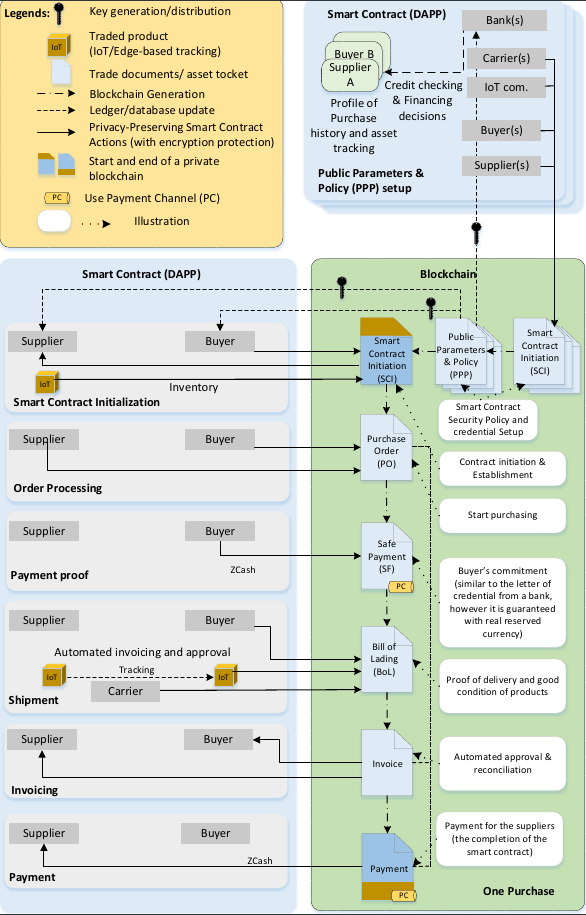
\includegraphics[scale=0.21]{supplychainexample.png}
\caption{A supply chain scenario using IoT devices, blockchain, and data encryption protections.}
\label{fig:supplychain}
\end{figure}
\end{frame}

\begin{frame}{Legends and Smart Contract interaction with Blockchain}
\begin{figure}[!ht]
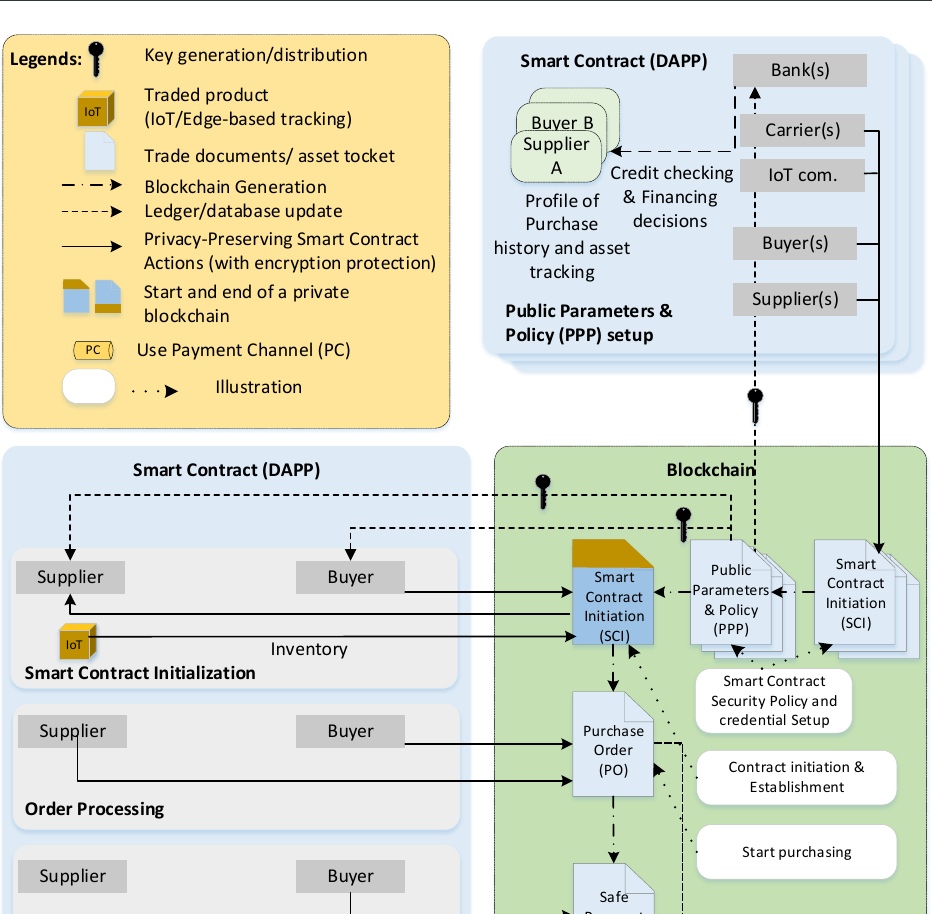
\includegraphics[scale=0.20]{supplychainlegendsscb.png}
\caption{Zoom-in on Legends and interaction of the first smart contract with the blockchain}
\label{fig:supplychainlegendsscb}
\end{figure}
\end{frame}

\begin{frame}{Smart Contract interaction with Blockchain}
\begin{figure}[!ht]
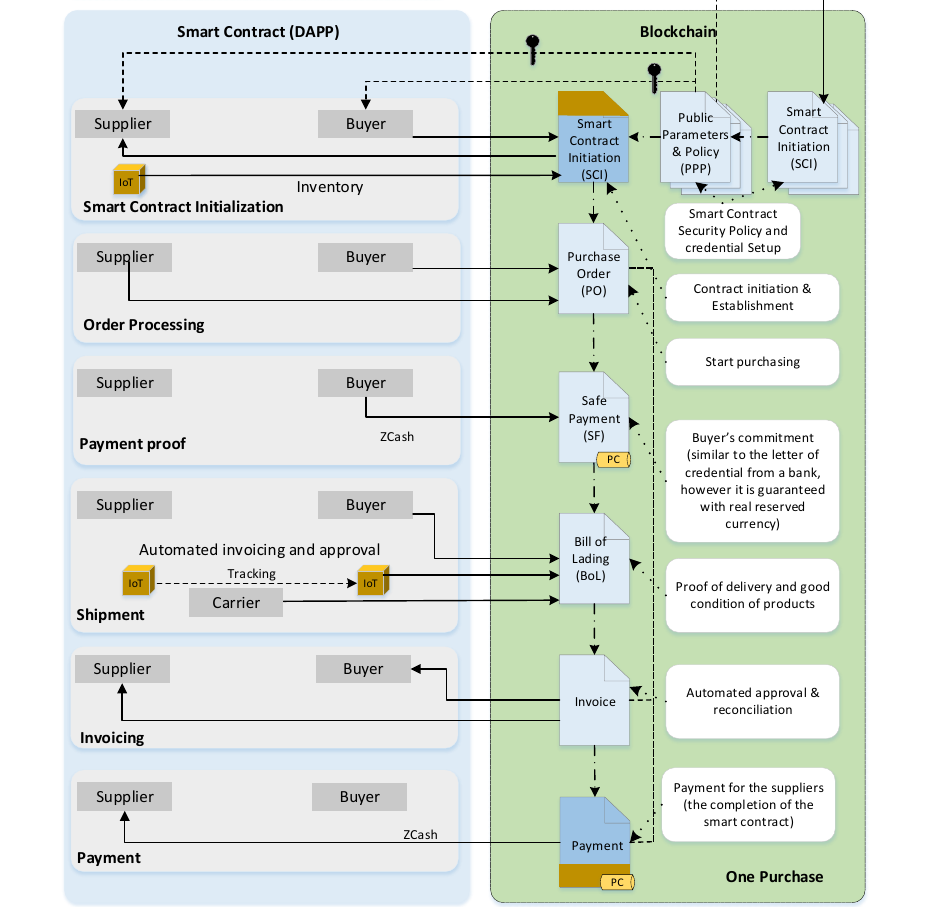
\includegraphics[scale=0.20]{supplychainscb.png}
\caption{Zoom-in on the interaction of the second smart contract with the blockchain}
\label{fig:supplychainscb}
\end{figure}
\end{frame}

\begin{frame}[allowframebreaks]{BCT-supported purchase related transaction using DApp}
The left side of the figure present a BCT-supported purchase related transaction by using Ethereum’s Decentralized App (DApp) solution involves 4 main procedures based on supply-chain operation procedures:
\begin{itemize}
\item \textbf{Order Processing}:
\begin{itemize}
	\item The order-processing workflow starts with a PO from the buyer. Within the blockchain, once created, the PO is time-stamped and can become a valid document whose clauses can be executed \textbf{only if valid}, due to the programming features of smart contracts.
	\item Assuming delivery documents can also be registered on it, the metadata of the invoice, PO and bill of lading could be matched automatically due to the smart contracts feature, which \textbf{ensures consistency between price and quantity} in all three documents (i.e. three-way-match), permitting an \textbf{automated} and \textbf{fast invoice approval}.
	\item The entire history of the transactions offers \textbf{perfect audibility}, and \textbf{trust between parties} is provided by the \textbf{immutability of the data} entered in a blockchain.
\end{itemize}	  

\item \textbf{Shipment}:
\begin{itemize}
	\item \textbf{IoT-based tracking capability} is a critical component for this procedure.
	\item Keeping track of the \textbf{material flow} at each step, along with the corresponding \textbf{paper flow}, is a major undertaking that \textbf{requires manual processes} that are subject to \textbf{human error}, \textbf{loss}, \textbf{damage} or even \textbf{theft} and \textbf{fraud}.
	\item Another potential application is provided by smart contracts and cryptographic multi-signatures and product content protection for all the various documentation and processing stages involved in a trade transaction.
	\item In such a blockchain-based IoT, there is the possibility of maintaining \textbf{product information}, its \textbf{history}, \textbf{product revisions}, \textbf{warranty details} and \textbf{end of life}, transforming the blockchain into a distributed and trusted blockchain.
\end{itemize}


\item \textbf{Invoicing}:
\begin{itemize}
	\item Blockchain-based services can register the invoice-related information on a blockchain in order to \textbf{avoid} \textbf{duplicates} and \textbf{fraud} across the network.
	\item As explained by \cite{hofmannstrewebosia}, each invoice would be distributed across the network, hashed and time-stamped in order to create a \textbf{unique identifier}.
	\item If a supplier tried to sell same invoice again through the network, that invoice would indicate a previous instance of financing to all parties, and the \textbf{double financing would be avoided}.
	\item The \textbf{integration with the payment system} is given by the ability of smart contracts to \textbf{take control over an asset} registered on a blockchain (e.g. crypto-cash) and \textbf{automatically trigger the payment}.
\end{itemize}

\item \textbf{Payment}: 
\begin{itemize}
	\item Developed to create a purely peer-to-peer version of electronic
cash to allow online payments, \textbf{payments are the first application of BCT}.
	\item With the use of Bitcoin or similar cryptocurrencies in a B2B scenario, buyer and supplier could \textbf{transact without any intermediaries} (e.g. banks) and with \textbf{very small transaction fees}.
	\item Blockchain solutions could create \textbf{more efficient payment processes} between banks, eliminating the need for each institution to \textbf{maintain} and \textbf{reconcile their own ledger}.
\end{itemize}

\end{itemize}

\end{frame}

\begin{frame}[allowframebreaks]{Privacy problem}
\begin{itemize}
\item The described smart contract \textbf{does not provide privacy protection} for transaction contents processed by smart contracts.
\item Two additional modules (incorporated into original supply-chain procedures):
\begin{enumerate}
	\item \textbf{Smart contract initialization}: 
	\begin{itemize}
		\item sets up the initial smart contract credentials such as agreed data access control policies for each step of smart contract;
		\item initiates the off-chain operation, in which we start a private blockchain at this point.
	\end{itemize}
	\item \textbf{Payment proof}:
	\begin{itemize}
		\item the private chain can also incorporate public blockchain evidence into the private blockchain;
		\item the addition of the payment proof procedure is to utilize the payment channel feature of public blockchains to \textbf{prove the buyer has sufficient money} to pay for the purchased product;
		\item  the buyer first pays for the product to a Escrow account, and once the product is landed, the cashed money will be delivered to the supplier to close the blockchain based purchase.
	\end{itemize}
\end{enumerate}
\end{itemize}
\end{frame}

\begin{frame}[allowframebreaks]{Smart Contracts}
\begin{itemize}
\item In Bitcoin, the concept of \textit{“scripting”} has already existed, which is actually \textbf{a weak version} of smart contract.
\begin{itemize}
	\item it lacks Turing-completeness, thus does not nearly support everything;
	\item it is value-blinded;
	\item it lacks state, UTXO can either be spent or not, there is no way to keep other states except for these two;
	\item it is blockchain blinded.
\end{itemize}
\item Ethereum smart contract is to build a decentralized application to create a blockchain with a build-in Turing complete programming language.
\item Smart contract means is defined to be a cryptographic “boxes” that contain value and only unlock it if certain conditions are met.
\item A smart contract will also be stored in the blockchain and can be retrieved by its address and integrity can be guaranteed as well.
\item With smart contract, one can express logics such as “only after April 17th, 2018, can the document be sent to A”.
\item In the presented supply-chain example in Figure \ref{fig:supplychain}, two smart contracts are involved:
	\begin{enumerate}
	\item \textbf{public blockchain smart contract}: the smart contract on the right side box includes multiple stake holders providing supply-chain services to settle down a \textbf{PPP} (Public Parameters and Policies).\\A PPP describes what encryption \textbf{public parameters} will be used for \textbf{data privacy protection}, who may serve as a \textbf{trusted party} for \textbf{data access control management} for running private blockchains, and what \textbf{security policies to be enforced} in the private blockchain. \textbf{We can treat PPP as a template};
	\item \textbf{private blockchain smart contract}: the smart contract on the left side of Figure \ref{fig:supplychain} represents a one purchase between a supplier and a buyer. In addition, an \textbf{IoT company} can be involved to provide \textbf{product tracking and inventory}.
	\end{enumerate}
\end{itemize}
\end{frame}

\begin{frame}{ABE-Enabled ABAC}

\end{frame}

\section{PoP System Models}
\begin{frame}{PoP System Models}
\begin{itemize}
	\item PoP System Models
\end{itemize}
\end{frame}

\section{PoP Operation and Performance Analysis}
\begin{frame}{PoP Operation and Performance Analysis}
\begin{itemize}
	\item PoP Operation and Performance Analysis
\end{itemize}
\end{frame}

\section{Summary}
\begin{frame}{Summary}
\begin{itemize}
	\item Summary
\end{itemize}
\end{frame}

\section{References}
\begin{frame}[allowframebreaks]{References}
\printbibliography
\end{frame}

\end{document}